\section{Clustering}
\subsection{Unsupervised learning introduction}
    Sometimes we do not have a training set with defined labels (results); therefore, we need to find some structure from the training set.
    \textbf{Clustering} is one way to do so, by grouping close data points together.


    Applications of clustering:
    \begin{itemize}
        \item Market segmentation.
        \item Social network analysis.
        \item Organize computer clusters.
        \item Astronomical data analysis.
    \end{itemize}

\subsection{K-means algorithm}
    K-means algorithm performs clustering by defining a "centroid" for each cluster and improve the accuracy of centroids through minimizing the total squared distances from the centroid to all points in the particular cluster.

    \begin{enumerate}
        \item Input: 
            \begin{itemize}
                \item $K$ (number of clusters).
                \item Training set ${x^{(1)}, x^{(2)},x^{(3)}, \dots x^{(m)})}$. $x^{(i)} \in \mathbb{R}^n$ (We drop the $x_0 = 1$ convention.
            \end{itemize}
        \item \textbf{Algorithm} The K-means algorithm has three main steps:
            \begin{enumerate}
                \item \textbf{Initialization}: Initialize cluster centroids (random).
                \item \textbf{Cluster Assignment}: (Loop: for all data points $x$) assignment of each data point into a cluster, depending on the proximity to the cluster centroid.
                \item  \textbf{Move Centroid}: (Loop: for all clusters) refine the centroid of each cluster by taking the mean location of all data points for an individual cluster.
            \end{enumerate}
            \begin{algorithm}[H]
            \caption*{K-means Algorithm}
            \begin{algorithmic}
                \STATE  Randomly initialize $K$ cluster centroids $\mu_1, \mu_2, \dots, \mu_K \in \mathbb{R}^n$ 
                \STATE \textbf{Repeat} \{
                \bindent
                \FOR{i=1 to m}
                \STATE $c^{(i)} := k$, s.t. $\min_{k} \| x^{(i)} - \mu_k \| ^2 $ \\
                \COMMENT {\textbf{Cluster assignment}: index ($ 1 \dots K$) of cluster centroid closest to $x^{(i)}$}
                \ENDFOR
                \eindent
                \\ 
                \bindent
                \FOR{k= 1 to K}
                \STATE $\mu_k$ := mean of points assigned to cluster k \\
                \COMMENT{\textbf{Move centroid}}
                \ENDFOR
                \eindent

            \STATE \}
            \end{algorithmic}
            \end{algorithm}
        \item K-means for non-separate clusters: sometimes the clusters are not well defined (separated enough). The algorithm will still produce clustering based on the proximity. An example is the \textbf{T-shirt sizing problem} (See Figure \ref{fig:t-shirt-sizing}) : for a given set of weight-height distribution from market survey, how many sizes should the manufacturer produced (S, M, L) or (XS, S, M, L, XL)?
    \end{enumerate}
    \begin{figure}[htpb]
        \centering
        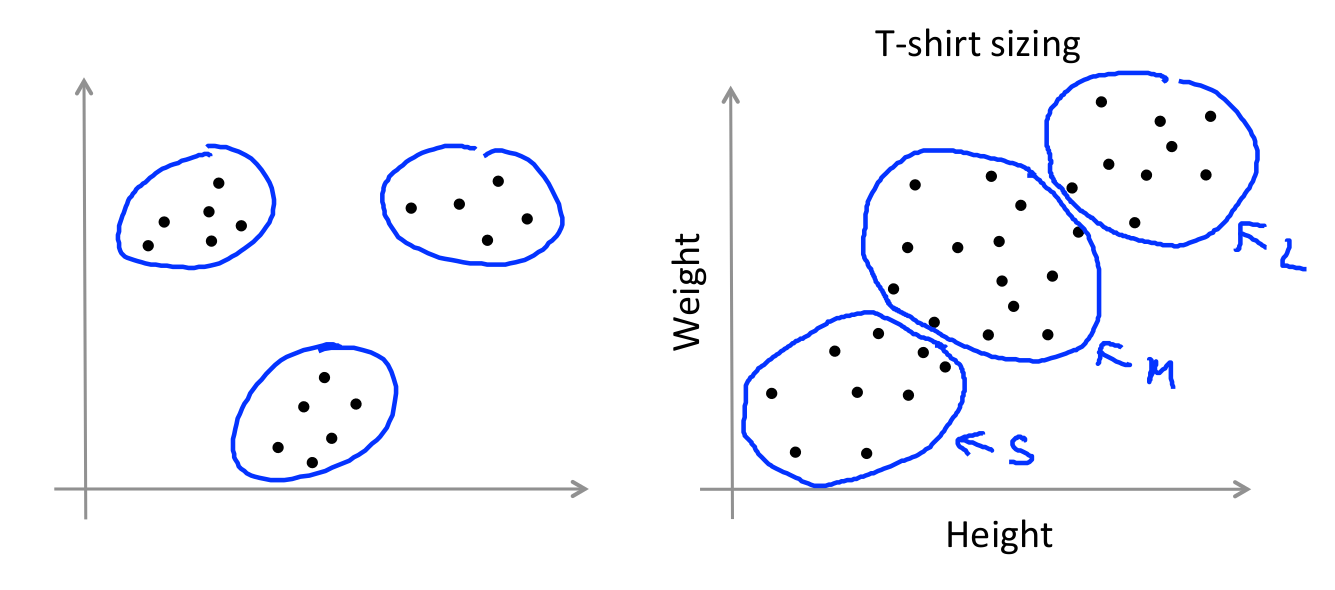
\includegraphics[width=0.8\textwidth]{image/t-shirt-sizing.png}
        \caption{Non-separated clusters: T-shirt sizing}
        \label{fig:t-shirt-sizing}
    \end{figure}
\subsection{Optimization Objective}
    \begin{enumerate}
        \item $c^{(i)}$ = \textbf{index}of cluster (1, 2, $\dots K$) to which example $x^{(i)}$ is currently assigned.
        \item $\mu_k$ = cluster centroid k. [Coordinate $\mu_k \in \mathbb{R}^n$]
        \item $\mu_{c^{(i)}}$ = cluster centroid of cluster to which example $x^{(i)}$ has been assigned.
        \item \textbf{Optimization objective}: \\
            \begin{equation}
                \min_{ \{c^{(i)}\}, \{\mu_k\} } J ( \{c^{(i)}\}, \{\mu_k\} )
                \label{eq:k-means-objective}
            \end{equation}
           \begin{equation}
                J ( \{c^{(i)}\}, \{\mu_k\} ) = \frac{1}{m} \sum_{i=1}^{m} \| x^{(i)} - \mu_{c^{(i)}} \|^2
               \label{eq:k-means-cost}
           \end{equation} 

           Note:
           \begin{enumerate}
               \item The first for loop in the algorithm (i) minimizes $J(\dots)$ with respect to $c^{(i)}$ and holds $\mu_k$ constant.
               \item The second for loop in the algorithm (k) minimizes $J(\dots)$ with respect to $\mu_k$ and holds $c^{(i)}$ constant.
           \end{enumerate}

    \end{enumerate}
\subsection{Random Initialization}
    Rules:
    \begin{enumerate}
        \item $K$ < m (number of training examples).
        \item Randomly pick $K$ training examples.
        \item Set $\mu_k$ to the K examples chosen in the previous step.
    \end{enumerate}

    There might be different clustering based on different initial random selection. Therefore one can run the K-means algorithm multiple times (100), each with a different random initialization (selection of examples as initial centroids). Compute all cost function (distortion), then pick the one that gives the lowest cost J.

\subsection{Choosing the number of clusters ($K$)}
    Sometimes it is ambiguous how many clusters there are, e.g. could be 2 or 4. One method of determining the number of clusters is the \emph{Elbow method}. We compute the cost and vary $K$- we will usually see a sharp drop in cost at the star, and the decreasing rate tends to slow down after the "elbow points". The elbow point is the point where the cost function's slopes magnitude starts decreasing. 

    \par However, not all scenario will produce an obvious "elbow" (refer to the graph on the right in Figure \ref{fig:elbow-method}). In such cases, the Elbow method doesn't give much insight.

    \begin{figure}[htpb]
        \centering
        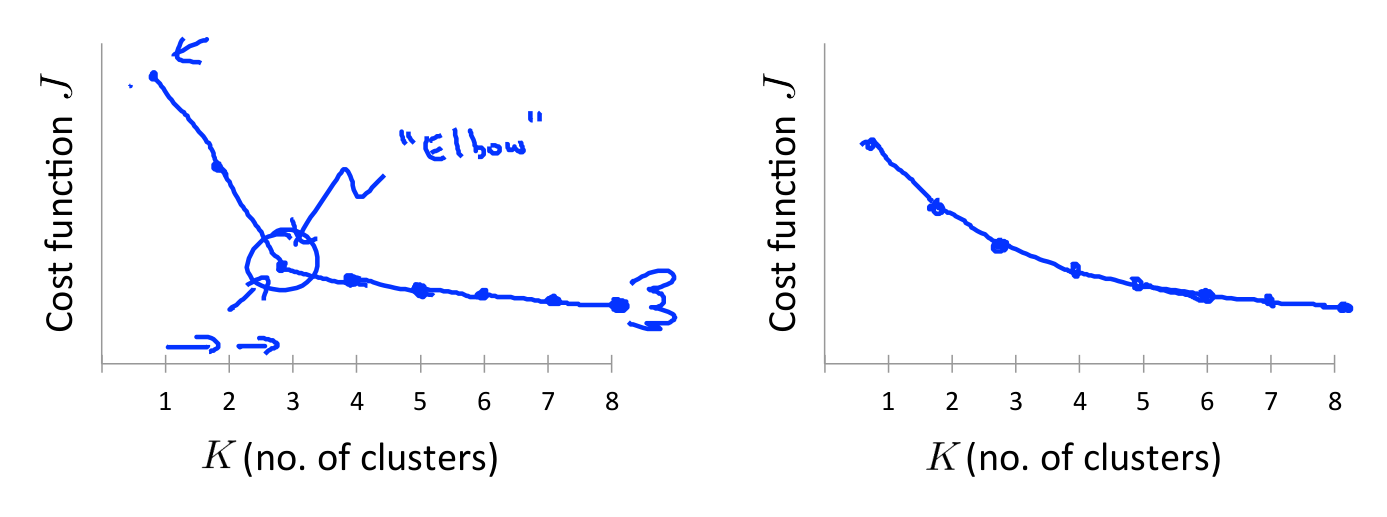
\includegraphics[width=\textwidth]{image/elbow-method.png}
        \caption{Elbow method in apparent cases (left) and non-apparent cases(right)}
        \label{fig:elbow-method}
    \end{figure}

    \par In some cases, there will only be some definitive $K$s to choose from. This is often seen in K-means based on a metric for some downstream purpose. Recall the T-shirt sizing problem, in such cases, we have standard numbers of clusters (3, 5, 7, etc.). One can then iterate through all possible options, and proceed with the one which yields the lowest cost.
